\section{Continuous exposure until the casing is uncovered}
The moving-wall calculation gives about 104--107 s for the sustainer and
138--142 s for the booster under the nominal continuous load. It advances the
gas-facing radius until it reaches the casing. Char can remain after the
virgin resin has decomposed, so conversion and casing exposure occur at
different times. This is an independent finite-volume calculation. ANSYS
verification of this coupled moving wall remains open.
\begin{table}[H]\centering
\begin{tabular}{lrrrr}\toprule
Case & Initial liner & Nominal event & Property flag & Film scenarios\\
 & [mm] & [s] & [s] & [s]\\\midrule
Sustainer Al & 4.7625 & 106.8 & 49.0 & 58.3--200.1 \\
Sustainer CF & 4.7625 & 103.9 & 20.5 & 56.5--194.9 \\
Booster Al & 6.3500 & 142.4 & 82.0 & 77.8--266.3 \\
Booster CF & 6.3500 & 137.7 & 35.1 & 74.7--258.3 \\
\bottomrule\end{tabular}
\caption{Nominal and film endpoints use 640 liner and 160 casing cells with
a 0.02 s step ceiling. Film scenarios change the uncorrected coefficient from
2000 to 500 W/(m$^2$ K), respectively. The other inputs retain nominal values.
The property flag in this table belongs to the nominal case.}
\end{table}
All events occur after the assumed intact casing exceeds its provisional
property range. The nominal gas temperature is 2504 K, nominal chamber pressure
is 800 psi, and the nominal uncorrected film coefficient is 1000 W/(m$^2$ K).
The calculation exposes the liner at ignition and sustains heating until full
local loss. Zero hot-side radiation is assumed at nominal conditions. The
outside sees a 22~$^\circ$C environment, an 8 W/(m$^2$ K) film and emissivity 0.25.
The extent of actual in-motor exposure is unknown.

The largest one-factor changes in this study come from wall heat transfer and
the assumed energy cost of char removal. The times in the last column compare
two specified heat-transfer scenarios. They do not quantify firing-to-firing
variability or a safe firing interval. Firing heat flux versus time and
recession measurements on the manufactured liner would directly constrain
the two inputs driving this spread. Section~\ref{sec:almelt} shows how accounting
for aluminium melting changes the liner times and when the backing melts.

\clearpage\section{Remaining thickness and casing heat-up}
\begin{figure}[H]\centering
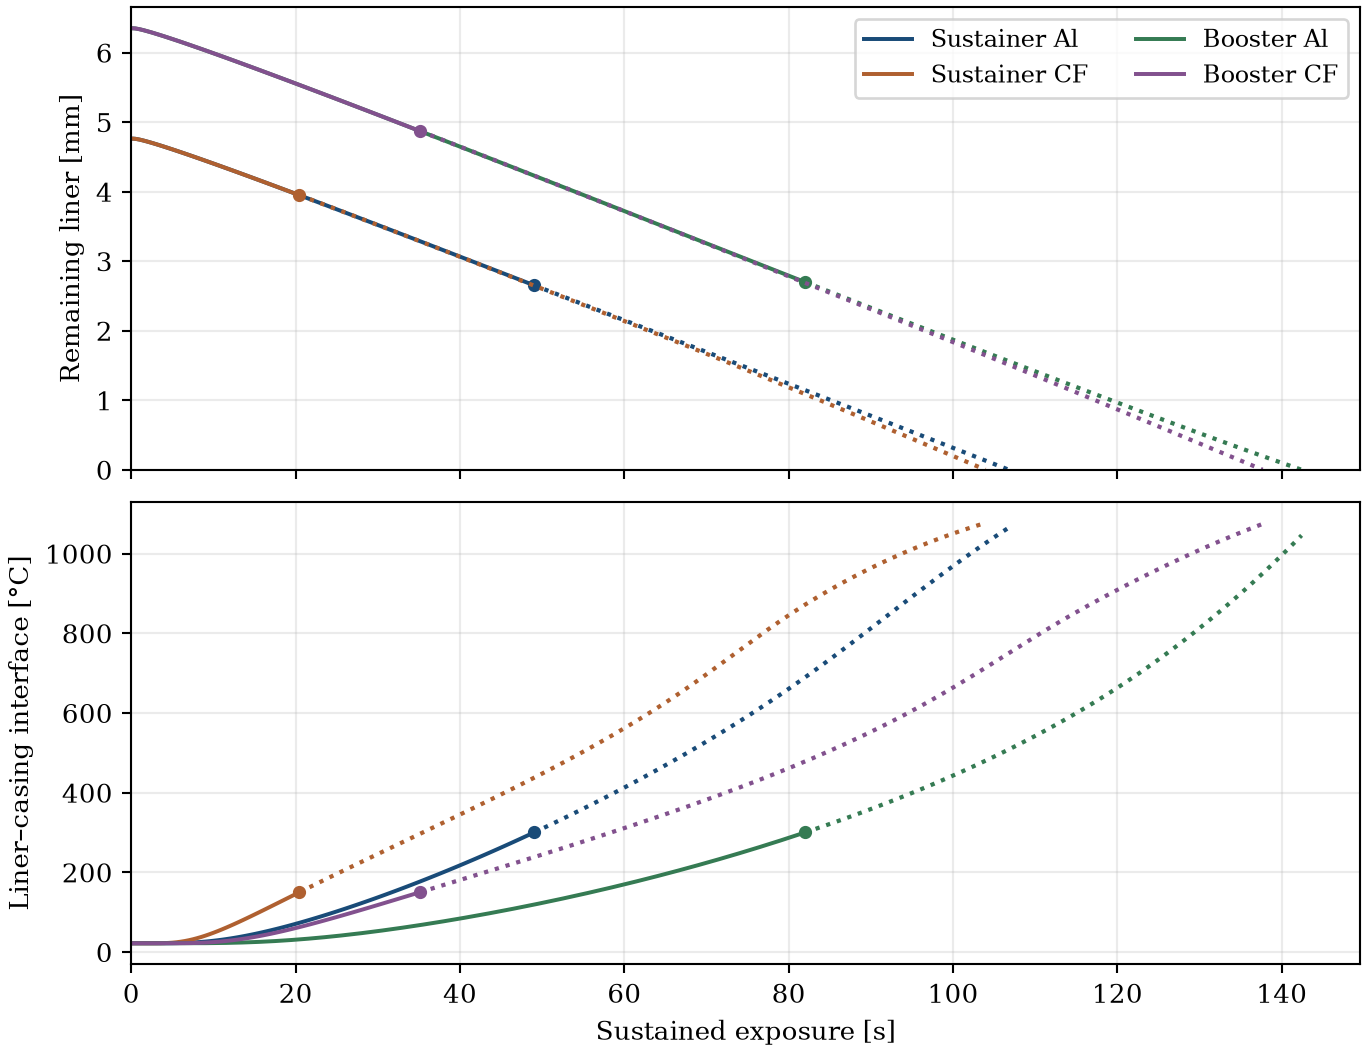
\includegraphics[width=.96\textwidth]{../analysis/moving_nominal.png}
\caption{Moving-wall calculation at the finest nominal setting. Dots mark the
first 150~$^\circ$C CF or 300~$^\circ$C Al property flag. Dotted lines continue
with the inherited backing properties. The horizontal axis measures continuous
exposure of the local wall.}
\end{figure}
The two casings give similar early surface recession because the heat initially
penetrates only partway through the liner. The model separates them more
clearly later as the casing absorbs heat. Each property flag denotes the
limit adopted for using those casing data. It does not identify loss of
pressure containment.

\clearpage\section{Temperatures, mass and energy in the sustainer Al calculation}
\begin{figure}[H]\centering
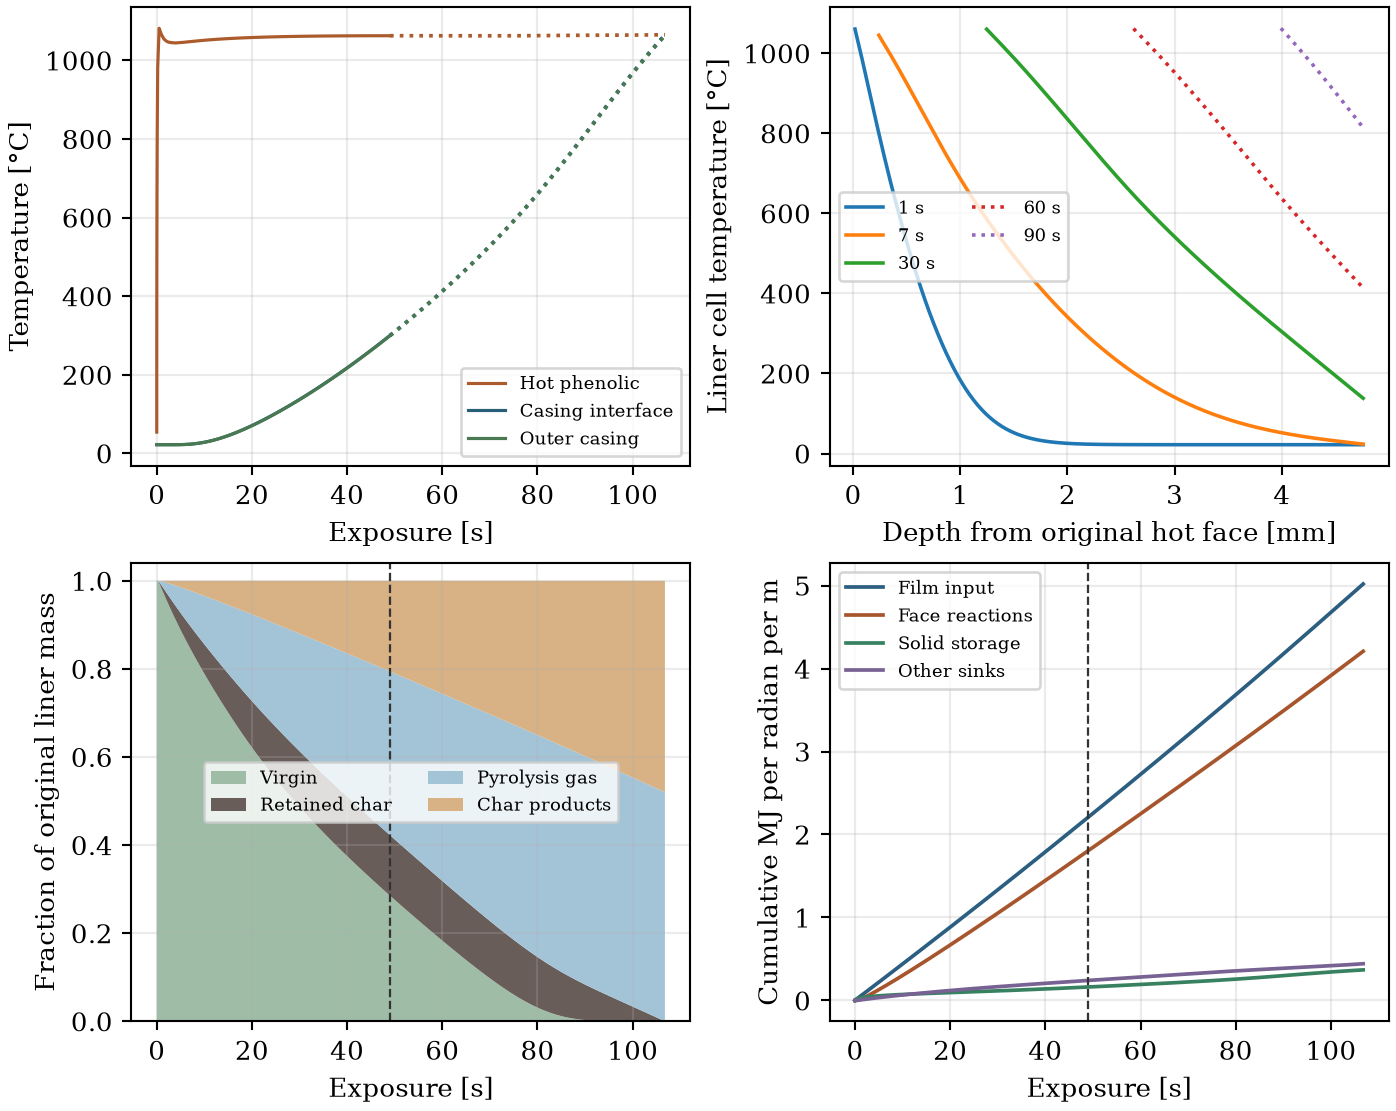
\includegraphics[width=\textwidth]{../analysis/moving_fields.png}
\caption{Upper panels show the three wall temperatures and the spatial
temperature profiles of the surviving liner. Profiles start at the first cell
centre. Lower panels account for the original liner mass and cumulative
energy. Dashed vertical lines mark the casing property flag; subsequent values
use surrogate continuation.}
\end{figure}
At 7 s the coupled wall gives 1048~$^\circ$C at the hot phenolic face and
0.235 mm removed. At the same exposure time the accepted earlier native
320-row sustainer Al calculation gives 1444~$^\circ$C at its live face and
0.045 mm of removed mesh. The gas is 2230.85~$^\circ$C in both cases.
The native calculation uses finite-row removal and its inherited reaction and
energy equations. This difference therefore includes changes to the model
as well as discretization; matching one final event time could conceal a
substantial difference in surface behaviour.

At nominal exhaustion the surface reaction terms account for 83.8 percent
of integrated film input in this case. The provisional 35 MJ/kg char cost
therefore warrants a direct sensitivity check. Swept sensible heat appears on
both sides of the interface accounting and cancels from the whole-wall ledger.

\clearpage\section{Numerical checks and open questions}
Twenty nominal calculations isolate the time step at 160 cells, double the
liner and casing radial counts twice at the same step, then halve the step on
the 640/160 mesh. The last two comparisons below use 320 to 640 liner cells at
0.04 s and 0.04 to 0.02 s at 640 cells.
\begin{table}[H]\centering\begin{tabular}{lrr r rr}\toprule
 & \multicolumn{2}{c}{Event shift [s]} & Thickness & \multicolumn{2}{c}{Mesh $\Delta T_s$ [K]}\\
\cmidrule(lr){2-3}\cmidrule(lr){5-6}
Case & Mesh & Time & diff. [mm] & All samples & From 0.5 s\\\midrule
Sustainer Al & -0.0019 & +0.0009 & 0.00016 & 30.3 & 2.4 \\
Sustainer CF & -0.0018 & -0.0003 & 0.00016 & 30.3 & 2.4 \\
Booster Al & -0.0032 & +0.0029 & 0.00024 & 39.3 & 4.7 \\
Booster CF & -0.0030 & +0.0000 & 0.00024 & 39.3 & 4.7 \\
\bottomrule\end{tabular}
\caption{Thickness difference is the largest across both comparisons at shared
times. The temperature columns give the greatest hot-face difference between
the two spatial resolutions, including or excluding the initial transient.}
\end{table}
All eight finest pairs meet the 5 percent event-time target and the
remaining-thickness target. Their final accepted time intervals overlap.
Three coarser pairs have disjoint intervals. A load applied instantaneously
to a massless reconstructed face gives a mesh-sensitive initial temperature.
The 640-cell result still requires a separate comparison with ANSYS under
matching equations, even where independent refinement differences are small.

The coupled implementation closes each cell energy equation before moving the
front. The accepted step limits conversion growth to 0.05 and surface travel
to 40 percent of the first-cell width while multiple cells remain. A remnant
below half the original pitch merges conservatively with its neighbour.
The last event is localized by solving for the step duration that brings
the radius to the interface. A manufactured isothermal char front reproduces
its analytical time to within $10^{-8}$ s at two resolutions. A nonuniform
reacting coupon, interrupted after mesh mergers and a property flag, gives
a byte-identical final state and history on restart. All twenty nominal
integrations close the cumulative open-system energy and mass ledgers to
relative residuals below $10^{-9}$ and $10^{-11}$, respectively.

\clearpage\section{One-factor sensitivity to assumed inputs}
Forty-two additional calculations each change one named input or one backing
material tuple at 320/80 cells and a 0.04 s step ceiling. The columns show
paired event times in the same order as their listed inputs, in seconds.
\begin{table}[H]\centering\begin{tabular}{lrrrr}\toprule
Case & Pressure & Radiation & Removal cost & Gas excess\\
 & 600 / 1000 psi & 0.1 / 0.3 & 17.5 / 70 MJ/kg & 0.9 / 1.1\\\midrule
Sustainer Al & 109 / 105 & 92 / 73 & 68 / 181 & 127 / 92 \\
Sustainer CF & 106 / 103 & 90 / 71 & 65 / 179 & 124 / 89 \\
Booster Al & 145 / 140 & 123 / 97 & 91 / 242 & 170 / 123 \\
Booster CF & 140 / 136 & 119 / 93 & 85 / 238 & 164 / 118 \\
\bottomrule\end{tabular}\end{table}
Radiation entries specify effective hot-side emissivity at the inherited gas
radiative temperature. Gas excess scales the 2208.85 K difference between
nominal gas and the initial wall, with convection coefficient and all other
parameters fixed. The gas probes measure local sensitivity. Pressure enters
the empirical consumption law; the film coefficient stays independent.

For each case, doubling and halving the film coefficient produce respectively
the earliest and latest event in this screen. Both endpoints were rerun at
640/160 and 0.04 s, then 0.02 s (sixteen checks). The largest individual time
shift is 0.007 s; 15 of sixteen pairs have overlapping final
intervals. All sixteen satisfy the event-change and shared-thickness criteria.
Individual endpoint intervals and the material crossings are recorded with
the cases. An alternative inherited carbon-composite property tuple shifts the
CF event by -0.84 s for the sustainer and -1.02 s for the booster. The
resin, layup, bond and grade used on the actual cases remain unspecified.

Sections~\ref{sec:almelt} and~\ref{sec:cfdiag} examine aluminium fusion and
CF resin decomposition with separate material surrogates.
\clearpage
